\documentclass [a4paper,12pt] {article}
\usepackage{fullpage}
\usepackage{graphicx}
\usepackage{hyperref}
\usepackage{color}

\begin{document}
\begin{titlepage}
	\begin{center}
		\textsc{\huge\\[5cm] COS 301 - Mini Project}\\[1cm]
		\textsc{\huge Functional requirements and application design}\\[1cm]
		\textsc{\huge Group 1B}\\[1cm]
		\textsc{\large 2015}
	\end{center}
\end{titlepage}
\tableofcontents
\pagebreak
\section{Group Information}
	\subsection{General Information}
	We used Github as our version control service. The repository can be accessed at: \linebreak \url{https://github.com/thinusn/Mini-Project-Requirements-Group-1B}
	\subsection{Group members}
	\begin{itemize}
		\item 13033922 Elzahn Botha
		\item 12223426 Estian Rosslee
		\item 13025105 Jaco-Louis Kruger
		\item 13073878 Daniel Araüjo
		\item 13093500 Paul Engelke
		\item 13028741 Frikkie Snyman
		\item 13019602 Thinus Naude
	\end{itemize}
	\subsection{Contributions to project}
	\subsection*{Participation}
	Estian Rosslee (12223426) only attended the two 1-hour meetings we had, \textbf{he did not do any of the work presented in this document.} All other members of the group participated fully towards completing the project.
	\subsection*{Who did what}
		\begin{itemize}
			\item Planning: Everyone
			\item Use case prioritization: Everyone
			\item Services contracts: Daniel Araüjo, Thinus Naude, Paul Engelke and Frikkie Snyman
			\item Required functionality: Jaco-Louis Kruger and Thinus Naude
			\item Process specifcations: Elzahn Botha, Daniel Araüjo, Paul Engelke
			\item Domain Model: Frikkie Snyman
			\item Latex and Gitgub: Thinus Naude
		\end{itemize}
	\pagebreak
	\subsection*{Github contribution}
     %	\large\textbf{\colorbox{green}{IMAGE OF GITHUB CONTRIBUTIONS}}
	\begin{figure}[h!]
		\centering
		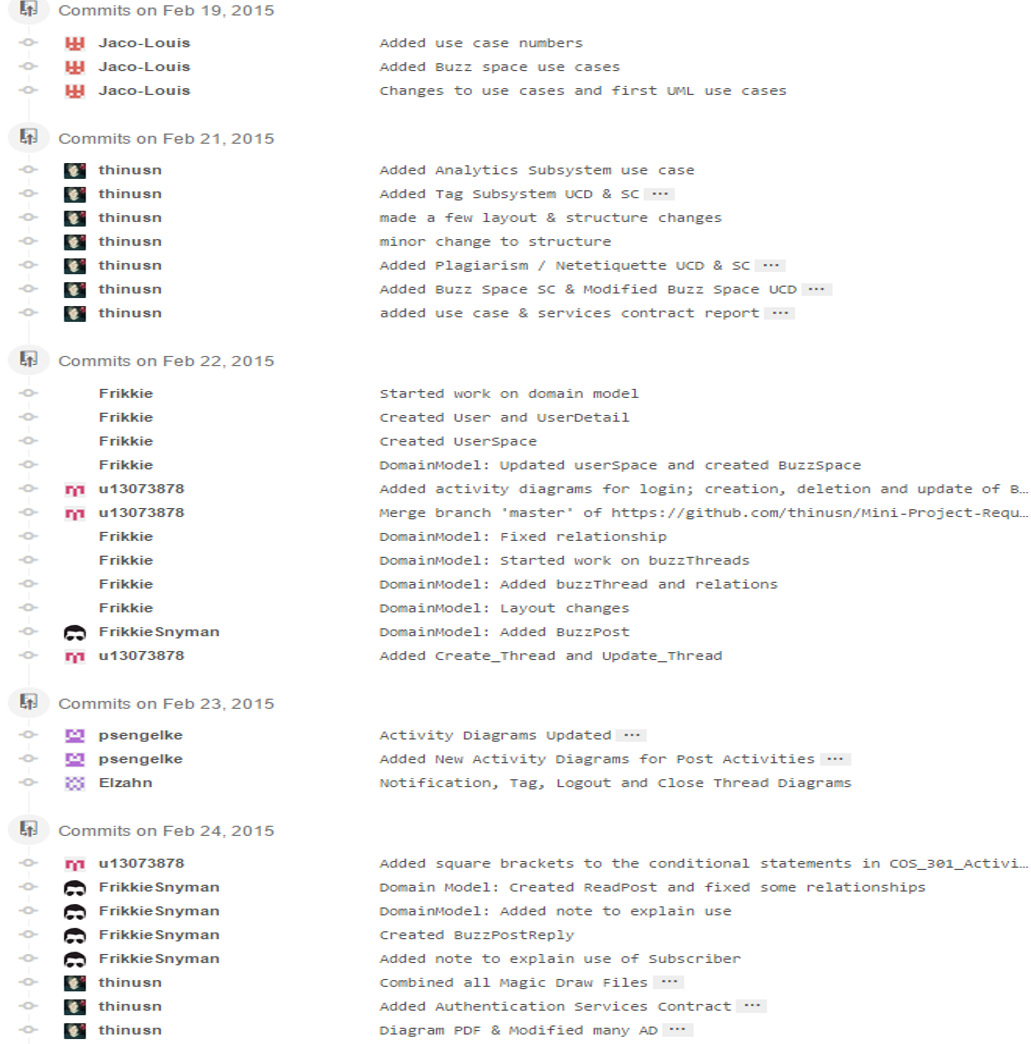
\includegraphics[width=0.95\textwidth]{githubCommits.png}
		\caption{Github pushes for project.}
	\end{figure}
\pagebreak
\section{Functional requirements and application design}
	\subsection{Use case prioritization}
	\subsection*{Critical}A use case which is absolutely essential
	\begin{itemize}
		\item Create, Read/View/Get, Delete and Update of BuzzSpace
		\item Create, Read/View/Get, Delete and Update of Thread
		\item Create, Read/View/Get, Delete and Update of Thread Posts
		\item Authentication	
	\end{itemize}
	\subsection*{Important}The system would still be useful without some of the important use cases, but the client would get quantifiably less value from the system.
		\begin{itemize}
			\item User (profiles and actions)
			\item User Communication (Email Templates)
			\item Tagging
		\end{itemize}
	\subsection*{Nice-To-Have}Its a requirement but the value to the clientis insignificant.
		\begin{itemize}
			\item Plagiarism checker
			\item Netiquette checker
		\end{itemize}

\pagebreak
	\subsection{Services contracts}
		\subsection*{Analytics}
			%\begin{figure}[h!]
			%	\centering
			%	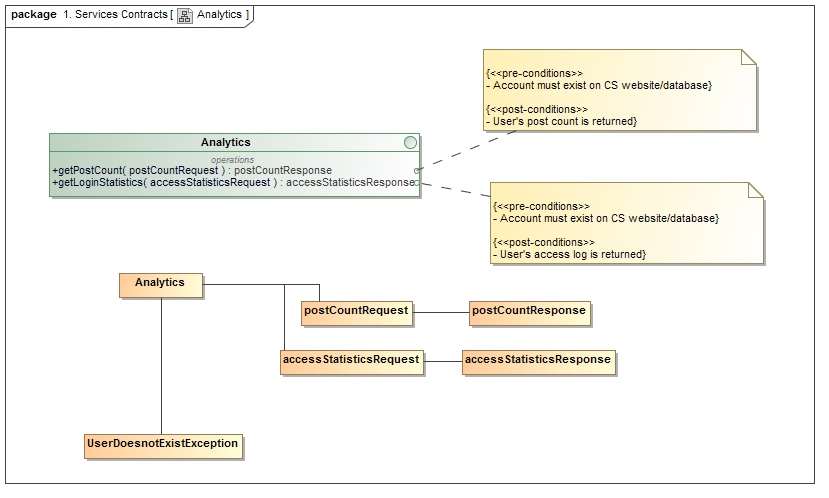
\includegraphics[width=0.95\textwidth]{AnalyticsSC.png}
			%	\caption{Analytics Services contracts.}
			%\end{figure}
		\subsection*{Authentication}
			\begin{figure}[h!]
						\centering
						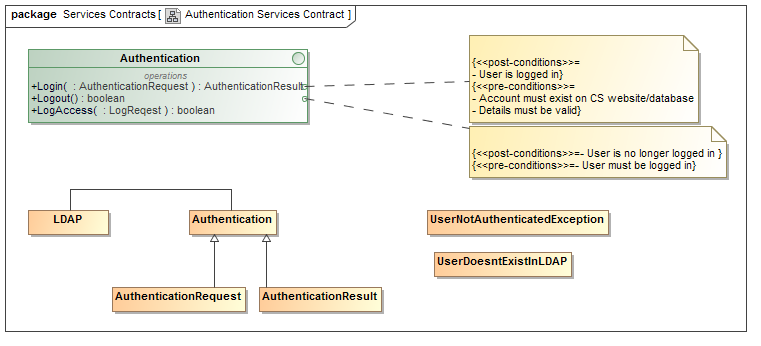
\includegraphics[width=0.95\textwidth]{AuthenticationSC.png}
						\caption{Authentication Services contracts.}
			\end{figure}
		\subsection*{BuzzSpace}
					\begin{figure}[h!]
						\centering
						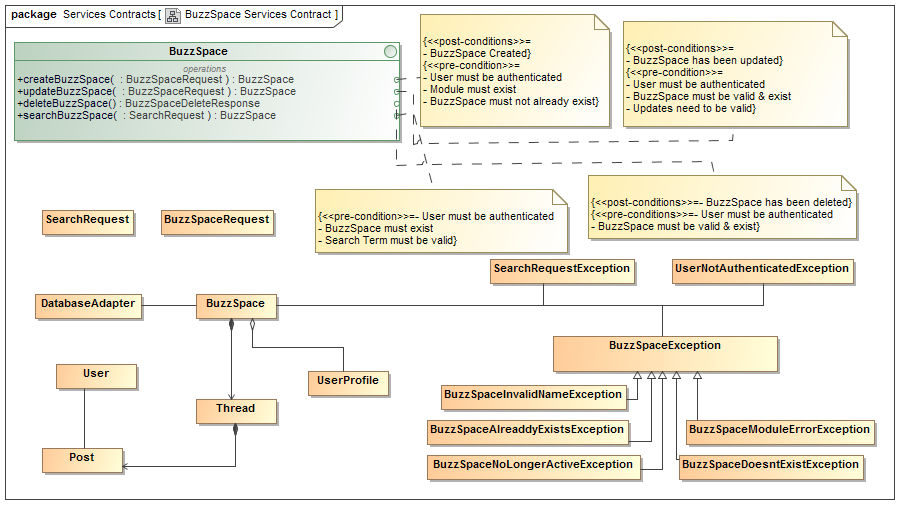
\includegraphics[width=0.95\textwidth]{BuzzSpaceSC.png}
						\caption{BuzzSpace Services contracts.}
					\end{figure}
		\subsection*{Communication}
		\subsection*{Plagiarism / Netetiquette}
		\begin{figure}[h!]
			\centering
			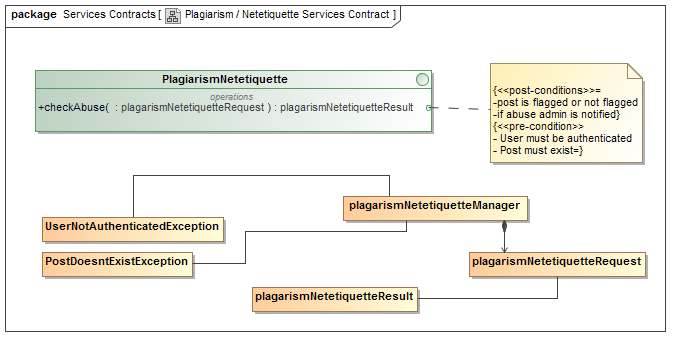
\includegraphics[width=0.95\textwidth]{PlagiarismNetetiquetteSC.png}
			\caption{Plagiarism and Netetiquette Services contracts.}
		\end{figure}
		\subsection*{Tagging}
			\begin{figure}[h!]
				\centering
				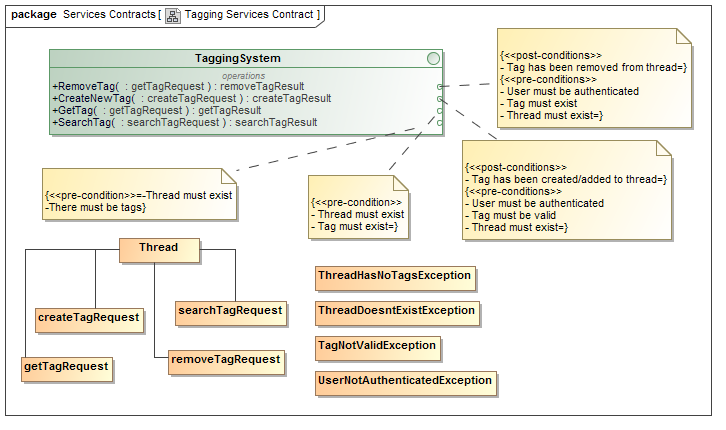
\includegraphics[width=0.95\textwidth]{TaggingSC.png}
				\caption{Tagging Services contracts.}
			\end{figure}
		\subsection*{Thread}
		\subsection*{Thread Posts}
		\subsection*{User}
\pagebreak
	\subsection{Required functionality}
		\subsection*{Analytics}
		\subsection*{Authentication}
		\subsection*{BuzzSpace}
		\subsection*{Communication}
		\subsection*{Plagiarism / Netetiquette}
		\subsection*{Tagging}
		\subsection*{Thread}
		\subsection*{Thread posts}
		\subsection*{User}
\pagebreak
	\subsection{Process specifcations}
		\subsection*{Analytics}
		\subsection*{Authentication}
		\subsection*{BuzzSpace}
		\subsection*{Communication}
		\subsection*{Plagiarism / Netetiquette}
		\subsection*{Tagging}
		\subsection*{Thread}
		\subsection*{Thread posts}
		\subsection*{User}

\pagebreak
	\subsection{Domain Model}
		\begin{figure}[h!]
			\centering
			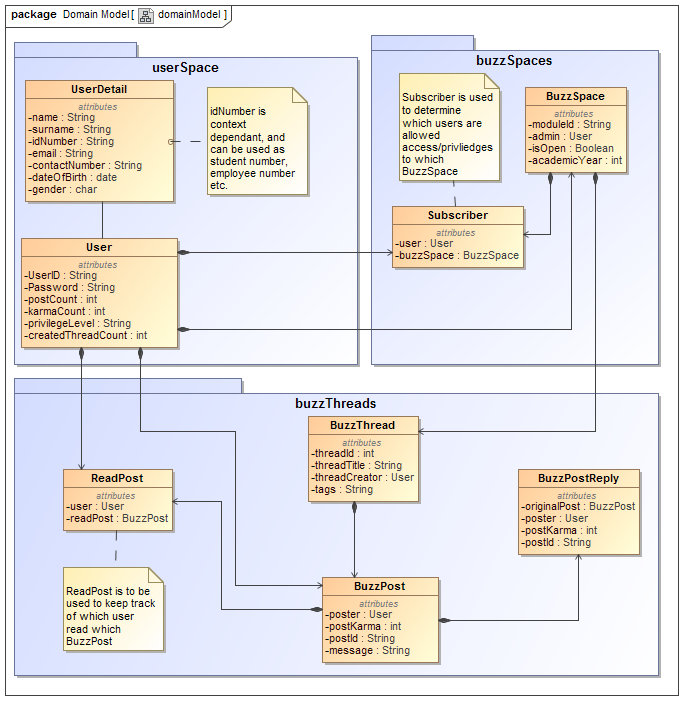
\includegraphics[width=0.95\textwidth]{domainModel.png}
			\caption{Domain model for the discussion board.}
		\end{figure}

\end{document}
